\documentclass[11pt]{jsarticle}

\usepackage{SPR}

\headerSPR
\begin{document}
	\titleSPR{\number\year}{\number\month}{\number\day}{D2}{吉田 皓太郎}
%%%%%%%%%%%%%%%%%%%%%%%%%%%%%%%%%%%%%%
	\articleSPRabst
		\begin{itemize}
			\item 機械学習を用いたカップ形状の設計支援
			\item 着後形状予測のためのカップの変形解析
		\end{itemize}
		
		
	\articleSPRobj
		\begin{enumerate}
			\item 定性的な機能要求を満たせるようなカップ形状を設計できる
			\item 布の物性とカップのパターンがどのような結びつきを持っているかを調べることができる.
		\end{enumerate}
%%%%%%%%%%%%%%%%%%%%%%%%%%%%%%%%%%%%%%
% 1.前回からのノルマ
	\articleSPRitemsone
		%\begin{enumerate}
		%	\item A
		%\end{enumerate}
		
		\tableofcontents
		
		
%%%%%%%%%%%%%%%%%%%%%%%%%%%%%%%%%%%%%%
%\begin{itemize}
%	\item 新規手法について
%	\item ISFAアウトライン
%\end{itemize}
%%%%%%%%%%%%%%%%%%%%%%%%%%%%%%%%%%%%%%
% 2.具体的な成果
	\articleSPRitemstwo
	\renewcommand{\labelitemi}{$\blacktriangledown$}
	%\renewcommand{\labelitemi}{$\bigcirc$}
	\newcommand{\argmax}{\mathop{\rm arg~max}\limits}
	\newcommand{\argmin}{\mathop{\rm arg~min}\limits}
	\newcommand{\Ker}{{\rm Ker}}
	\newcommand{\rank}{{\rm rank}}
%%%%%%%%%%%%%%%%%%%%%%%%%%%%%%%%%%%%%
	\section{研究進捗について}
		\subsection{設計者への示唆システム}	
			先日お話した可展面の修正システムにおいて,設計者が意図せず制約を破ってしまうことを事前に検知するシステムを構築した.
			
			考え方を示す.初めに,修正後の可展面における母線角,測地的曲率をそれぞれ$ \hat{\omega}_{\eta}, \hat{\alpha} $とする.この時,母線の最大長は$ EG-F^2 =0$の解によって与えられ,次式で表される.
			\begin{equation}\label{eq:DistMax}
				D_{\max} = \frac{\cos \hat{\alpha}}{\hat{\alpha}' + \hat{\omega}_{\eta}}
			\end{equation}
			自己交差の判定関数を$ f(s;\varepsilon_c)$とし,以下のように定める.
			\begin{equation}\label{eq:judgeFunc}
				f(s;\varepsilon_c) =
				\begin{cases}
				 |\xv_L + D\bd{g} + \varepsilon(s;\varepsilon_c)| - D_{\max}(s;\varepsilon_c) & if D_{\max}(s;\varepsilon_c)>0 \\
				 0 & else
				 \end{cases}
			\end{equation}
			このようにする理由は,$ D_{\max} $の増減方向は母線の方向に沿って決定されているためである.仮に$ t<0 $の場合には,母線と逆方向のところに特異点を持つことになる.$ t $の増減方向が大きく変化する場合,具体的には元の増減方向$ \bd{d}_{bt} $と変更後の方向$ \bd{d}_{at} $の内積が負になる場合,は場合分けが必要であると思われる.(要検討)
			今回は,二つの内積が正になる場合において考える.この時,設計者への示唆システムは以下のようにまとめられる.
			\begin{enumerate}
				\item $ s_{\max} = \argmax_{s\in [0,L_L]} f(s;\varepsilon_c) $を求める.
				\item $ f(s_{\max};\varepsilon_c) <0$ならば,母線の自己交差は起きず,実行可能であることを出力する.そうでなければ3に進む
				\item $ f(s_{\max};\varepsilon_c) = 0 $を満たす$ \varepsilon_c $を求める.これが設計者の意図する方向へ進めることができる最大値であるとして出力する.
			\end{enumerate}
			$ f(s;\varepsilon_c)$は厳密には不連続関数なので,二分法などの一般的な解法は諦め,$ \varepsilon_c $を徐々に減らしていくことによる全探索で求めることにした.
			
			計算結果比較
			\begin{figure}
				\begin{minipage}{0.5\hsize}
					\centering
					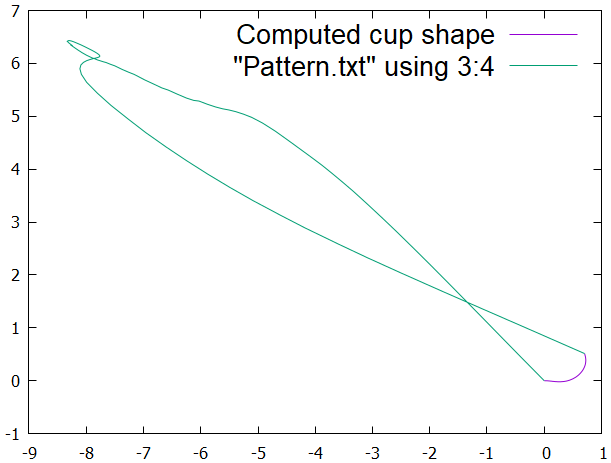
\includegraphics[width = \columnwidth]{./figure/CrossingData/Patt.png}
				\end{minipage}
				\begin{minipage}{0.5\hsize}
					\centering
					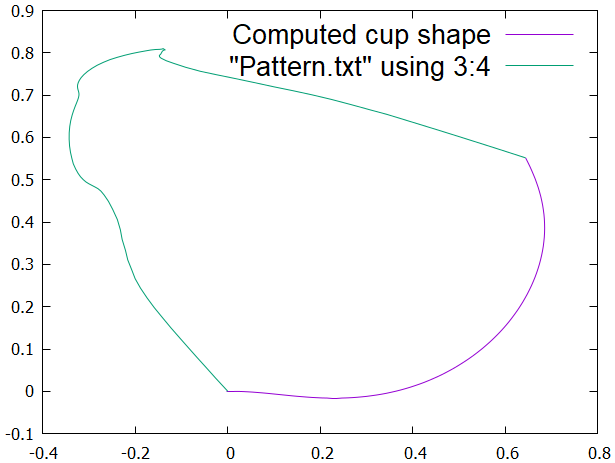
\includegraphics[width = \columnwidth]{./figure/test2/Patt.png}
				\end{minipage}
				\caption{$ \varepsilon_c $を大きく振りすぎた時の展開形状と,システムに基づき修正された展開形状}
			\end{figure}
			この方法では,ぎりぎり展開形状に異常がない程度のものを出力するため,少し曲線にがたつきがあったりするが,全体的には,交差を解消するような移動量を提案できたと結論づけられる.
	\newpage
\vspace{10cm}
%%%%%%%%%%%%%%%%%%%%%%%%%%%%%%%%%%%%%%
% 3.達成できなかったこととその問題点
	%\articleSPRthree
	
%%%%%%%%%%%%%%%%%%%%%%%%%%%%%%%%%%%%%%

\vspace{14cm}
%%%%%%%%%%%%%%%%%%%%%%%%%%%%%%%%%%%%%%
	\articleSPRfour
	\articleSPRfive
\end{document}
